\documentclass[12pt]{report}
\usepackage[pdftex]{graphicx}
\author{James Clements}
\date{Fall 2012}
\title{ME 351A: Inviscid Fluid Mechanics Notes}
\usepackage{textgreek}
\usepackage{ulem}
%\usepackage{fullpage}
\begin{document}
\maketitle
\tableofcontents
\chapter{What is a fluid? - 9/25/2012}
\begin{itemize}
\item Commonsense definition: fluids "fill their container", fluids "takes shape of container
\item Studying fluid mechanics requires more mathematical precision. 
\end{itemize}
\section{Mathematically precise definition of fluid}
(1) A fluid is a substance that deforms$^*$ continuously under the action of any shear$^*$ stress.

We will use continuum assumption to describe fluid flows. Namely, fluid/flow properties are continous and can be defined pointwise in space.

\begin{itemize}
\item[Consider:] A microscopic view of actual fluids
\begin{figure}[h]
\centering
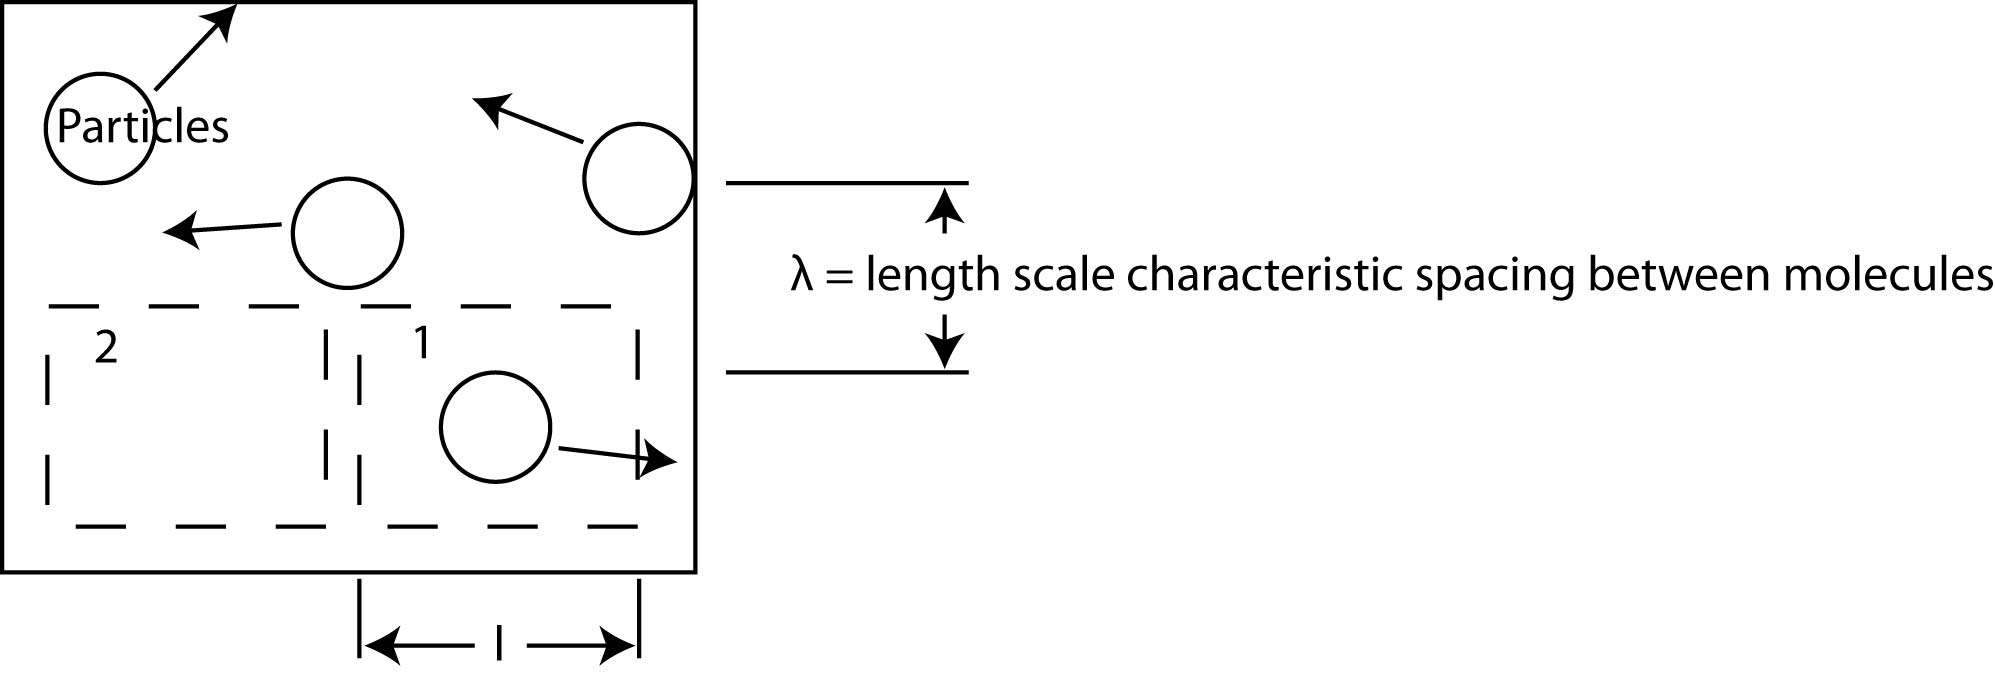
\includegraphics[width=100mm]{MicroscopicFluidExampleME351A.jpg}
\end{figure}
\item Individual particles undergo random motion in a fluid
\item[Suppose] You want to quantify the fluid density, \textrho : $\rho(\bar{x},t) $ which is a function of space and time.

If I use sampling windows spanning lxl:
\item $\rho \neq 0 $ in window 1
\item $\rho = 0$ in window 2
\item[Result: ] To study fluids at the macro level, assume that sampling windows span size l such that:
\[\lambda<<l<<\eta\]
where $\eta$ represents the smallest important scale of the flow system. This will keep my system continuous.
\item Note that $\eta$ is set by flow geometry
\item $\eta_{Gas}$ is between $10^{-7}$ and $10^{-8}$ meters

\item We need a $\lambda<<l$ so properties vary continuously
\item $l<<\eta$ is sued so we can discriminate variations in properties.

\item[In practice: ] do not need to actually define l for most engineering problems. Usually can be confident that such a scale exists. 

\item[\textbf{!Warning}] Might not be able to apply continuum assumption under the following cases:
\item Microfluidics can be problematic if $\eta$ is very small
\item Rarified systems (ie: in space), intermolecualar spacing, $\lambda$, might get very large. This can be a problem too.
\item Study of fluid at molecular scale is field on its own called Kinetic Theory or Physical Fluid Dynamics

\end{itemize}
\section{Fluid Properties}
\begin{itemize}
\item[Scalars:]
\item Zero order tensor
\item no directional information
\item time, t; pressure, p; density, $\rho$; kinematic viscosity $\nu$
\item[Vectors:]
\item Order 1 tensor
\item 1 item of directional information
\item 1 subscript associated with it.
\item Position $\vec{x}=($\b{x}$) =x_1\hat{e}_1 + x_2\hat{e}_2 + x_3\hat{e}_3 = x_i\hat{e}_i $; velocity $\vec{u}$, vorticity $\vec{\omega}$

Note: Einstein summation convention: sum over repeated indicies. 

Therefore: $x_i\hat{e}_i =\sum\limits_{i}x_i\hat{e}_i $

\item[Unit Vectors: ] Note that in Cartesian coordinates, unit vectors are: $\hat{i}, \hat{j}, \hat{k}$ for x,y,z directions respectively. For velocity, components are oriented in the u,v,w direction.

\item[2nd Order Tensors]
\item 2 directional components
\item 2 subscripts
\item Velocity gradient tensor $\nabla\vec{u} = \left(\nabla\vec{u}\right)_{ij}$ the $\nabla$ operator creates a tensor of order 1 higher than the initial variable.
\item[Note on Tensors: ] $\left(\nabla\vec{u}\right)_{ij}$ contains an i and a j component. i refers to the row and derivative operator. j refers to the column and velocity component. Expanded, the operator looks like this:

\[\nabla\vec{u} = \left(
\begin{array}{ccc}
\frac{\partial u_1}{\partial x_1} & \frac{\partial u_2}{\partial x_1} & \frac{\partial u_3}{\partial x_1} \\
\frac{\partial u_1}{\partial x_2} & \frac{\partial u_2}{\partial x_2} & \frac{\partial u_3}{\partial x_2} \\
\frac{\partial u_1}{\partial x_3} & \frac{\partial u_2}{\partial x_3} & \frac{\partial u_3}{\partial x_3} \\
\end{array}\right)\]

\item[\textbf{!Fact: }] for any general 2nd order tensor \uuline{A} can decompose as:
 \[\uuline{A} = \frac{1}{2}\left(\uuline{A}+\uuline{A}^T\right)+ \frac{1}{2}\left(\uuline{A}-\uuline{A}^T\right)\]
 
 \item For $\nabla\vec{u}$: we write: $\nabla\vec{u}=\frac{1}{2}\left(\nabla\vec{u}+\left(\nabla\vec{u}\right)^T\right)+\frac{1}{2}\left(\nabla\vec{u}-\left(\nabla\vec{u}\right)^T\right)=\uuline{S}+\uuline{\Omega}$

\[S_{ij} = \frac{1}{2}\left(\frac{\partial u_i}{\partial x_j}+\frac{\partial u_j}{\partial x_i}\right) \]
\[\Omega_{ij} = \frac{1}{2}\left(\frac{\partial u_j}{\partial x_i}-\frac{\partial u_i}{\partial x_j}\right) \]
\item Where S is the train rate tensor and $\Omega$ is the rotation rate tensor. 
\item Note that KUNDU defines these with a different notation. He has a different sign and multiplier.

\end{itemize}

\chapter{Types of Fluid Motion - 9/27}
\section{Understanding Velocity gradient tensor}


\end{document}